\chapter{Basic theory}

\section{The calculation grid}\label{Par:calc_grid}

%GEOtop is a distributed hydrological model capable of calculating the complete water and energy cycle in a domain, given the meteorological forcing in input. 
\subsection{Planar grid}
The calculation domain is based on a fixed regular Cartesian grid that coincides with the DEM (Digital elevation model), as reported in Fig. \ref{Fig_gen_dem}, on which it is possible to extract the hydrological basin closed at a given outlet  (Fig. \ref{Fig_dem_dxdy}). The X-axis coincides with the west-east direction and the Y-axis with the South-North direction, whereas the calculation grid size coincides with the pixel size (dX, dY) of the DEM. 


\begin{figure}[!h]
\begin{center}
\begin{minipage}[c]{1.0 \textwidth}
\centering
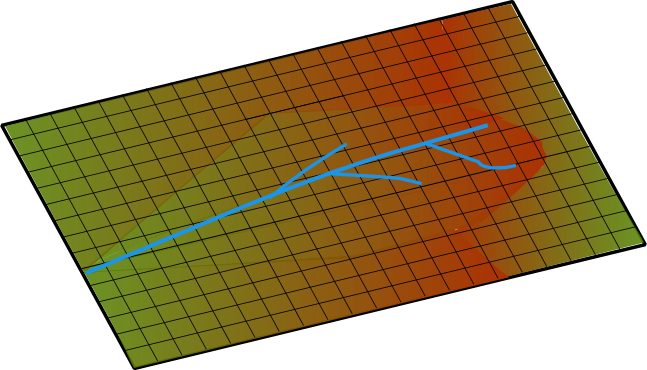
\includegraphics[width =0.72 \textwidth]{./images/pic_domain/dem_river}
\end{minipage}%
%\hspace{10mm}%
%\begin{minipage}[c]{0.46 \textwidth}
%\centering
%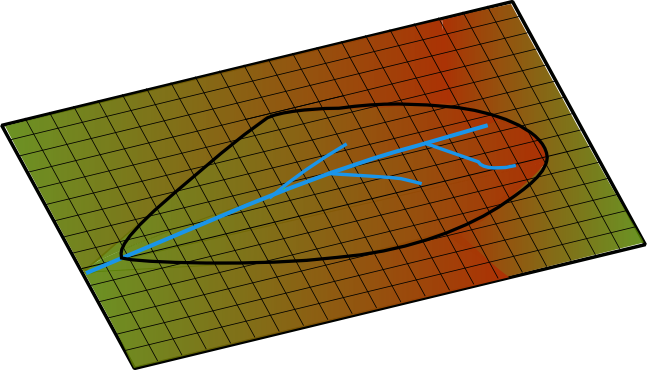
\includegraphics[width =1 \textwidth]{./images/pic_domain/dem_river_basin}
%\end{minipage}%
\end{center}
\caption{DEM of an the area of interest}
\label{Fig_gen_dem}
\end{figure}



\begin{figure}[tbp]
\begin{center}
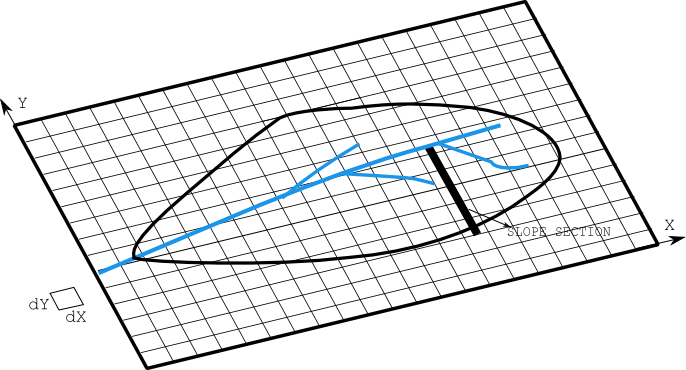
\includegraphics[width=0.7 \textwidth]{./images/pic_domain/dem_dxdy}
\caption{Calculation grid coinciding with the DEM. The hydrological basin (black line) and the river network (blue line) are present.}
\label{Fig_dem_dxdy}
\end{center}
\end{figure}

\subsection{Vertical grid}
The Z-axis is vertical and oriented towards the center of the Earth. It is possible to define the number of layers along the z-axis and the discretization, i.e. the vector of layer depths (Fig. \ref{Fig_discr3d} left). Note that the layer depth be irregular (different layers of various depths) but uniform in all the domain and the layer numbering starts from the top to the bottom (Fig. \ref{Fig_discr3d} right). The calculation grid points coincide with the center of the cell (on the X-Y axis) and the center of the layer (on the X-Z axis). Table \ref{table_vert_grid} reports and example of a vertical grid discretization characterized by 8 layers with irregular depths.

\begin{center}
\begin{longtable}{|p {1.5 cm}|p {2.2 cm}|}
\hline
\textbf{Layer ID} & \textbf{Depth (mm)}  \\ \hline
\endfirsthead
\hline
\multicolumn{2}{| c |}{continued from previous page} \\
\hline
\textbf{Layer ID} & \textbf{Depth (mm)} \\ \hline
\endhead
\hline
\multicolumn{2}{| c |}{{continued on next page}}\\ 
\hline
\endfoot
\endlastfoot
\hline
1 &10  \\ \hline
2 &15  \\ \hline
3 &20  \\ \hline
4 &20  \\ \hline
5 &60  \\ \hline
6 &50  \\ \hline
7 &80  \\ \hline
8 &100  \\ \hline
\caption{Vertical grid discretization and layer depth}
\label{table_vert_grid}
\end{longtable}
\end{center}



\begin{figure}[!h]
\begin{center}
\begin{minipage}[c]{0.46 \textwidth}
\centering
\includegraphics[width =0.9 \textwidth]{./images/pic_domain/discre_3d_nospess}
\end{minipage}%
\hspace{10mm}%
\begin{minipage}[c]{0.46 \textwidth}
\centering
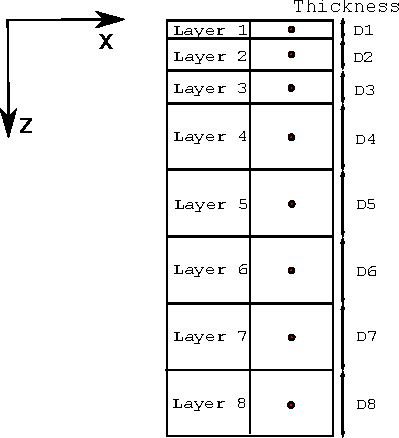
\includegraphics[width =0.9 \textwidth]{./images/pic_domain/soil_verticale.pdf}
\end{minipage}%
\end{center}
\caption{Left: three dimensional calculation grid. Right: discretization on the x-z plane. The red points, at the center of the cell, coincide with the calculation grid points}
\label{Fig_discr3d}
\end{figure}

\newpage
\begin{figure}[tbp]
\begin{center}
\begin{minipage}[c]{0.35 \textheight}
\centering
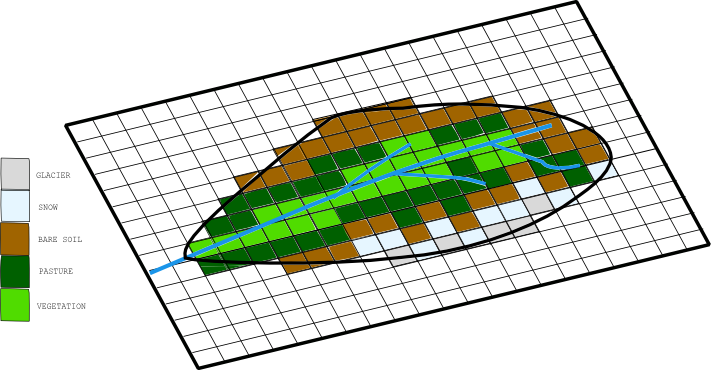
\includegraphics[width=1.4 \textwidth]{./images/pic_domain/land_cover_foglia}
\end{minipage}
\vspace{10 mm}
\begin{minipage}[c]{0.5 \textheight}
\centering
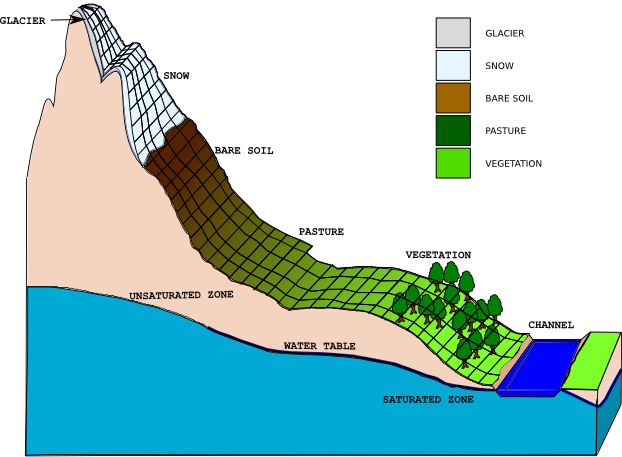
\includegraphics[width=0.9 \textwidth]{./images/pic_domain/general2D}
\end{minipage}
\caption{Top: Classification of a slope surface in a mountain basin on the basis of the land cover. Bottom: same classification for the entire basin.}
\label{Fig_general}
\end{center}
\end{figure}

\section{The domain characterization}

The domain characterization has the objective to determine:
\begin{itemize}
\item the land use i.e. vegetation, pasture, snow, glacier, forest etc. This map is usually called {\t land cover}
\item the stratigraphical characteristics of the soil, i.e. 1 m of thick debris (gravel), 2 m of sand, 2 m of loam etc. in order to ease the guess of the hydraulic and thermal parameters of the soil. This map is usually called {\it soil type}.
\end{itemize}


\subsection{Land cover}

Let us define a slope on the DEM, as reported in Fig. \ref{Fig_dem_dxdy}: ideally it can be figured out as in Fig. \ref{Fig_general}: at the bottom left is located the channel, then towards the higher elevations one may found the vegetated area, pasture, bare soil, snow covered area and glacierized area. 
%Inside the domain one may think about the water table, above which is the unsaturated zone and below which the saturated zone.
 Fig. \ref{Fig_general} on the top reports the slope surface discretization and classification, whereas on the bottom reports the land cover classification of the whole domain.
In this example may be identified five classes of land cover: vegetated area, located near the main stream in the low elevated range; pasture area, located in the medium range elevations; bare soil area, located on the steepest part of the domain and at medium-high elevations; snow covered area, located at high elevation and finally the glaciarized area on the highest parts.
% on the bottom.



\begin{figure}[tbp]
\begin{center}
\begin{minipage}[c]{0.35 \textheight}
\centering
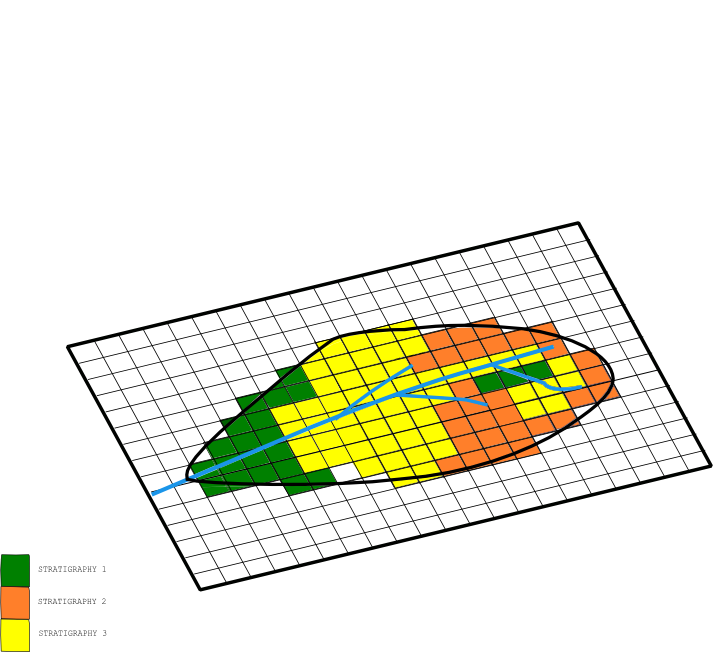
\includegraphics[width=1.3 \textwidth]{./images/pic_domain/soil_type_foglia}
\end{minipage}
\vspace{10 mm}
\begin{minipage}[c]{0.5 \textheight}
\centering
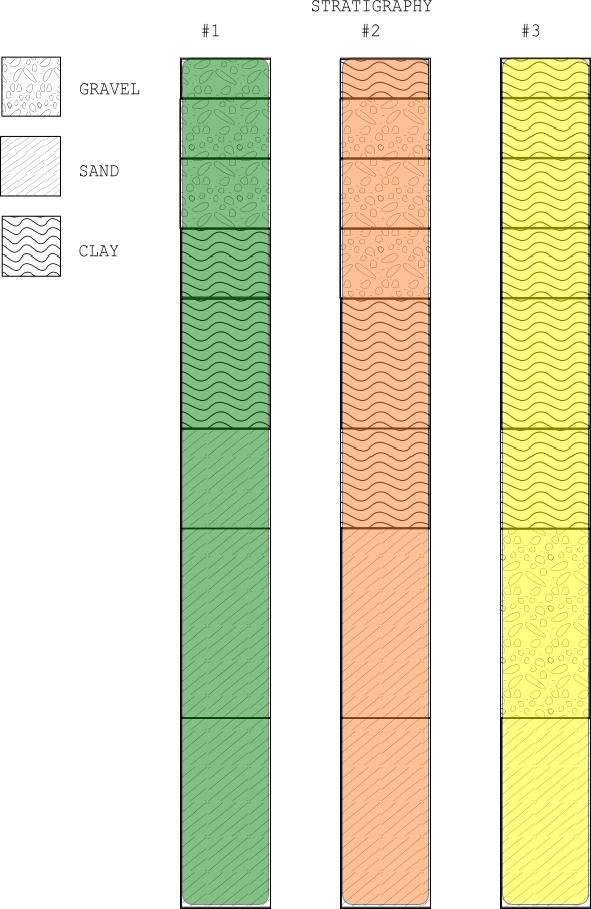
\includegraphics[width=0.5 \textwidth]{./images/pic_domain/1Dsoiltype.png}
\end{minipage}
\caption{Domain characterization oriented to define the soil stratigraphy (soil type map).}
\label{Fig_soiltype_foglia}
\end{center}
\end{figure}


\subsection{Soil type}

Let us imagine to take a section of the slope and to classify the type of soil in terms of texture (debris, gravel, sand, loam, clay) and bedrock depth. Each classification number would correspond to a particular soil stratigraphy, defining the soil particles and depth of bedrock. Starting from these characteristics, one could derive the hydraulic and thermal parameters, e.g. according to \citet{VanGenuchten1980, schaap2001rcp}. Fig. \ref{Fig_soiltype_foglia} reports the resulting map where each color corresponds to a given soil stratigraphy; the description of each type of soil stratigraphy is given in Table \ref{table_soil_type}.

\begin{center}
\begin{longtable}{|p {2.2 cm}|p {2.5 cm}|p {2.2 cm}|}
\hline
\textbf{Stratigraphy ID} & \textbf{Layer ID involved}   & \textbf{Soil texture}  \\ \hline
\endfirsthead
\hline
\multicolumn{3}{| c |}{continued from previous page} \\
\hline
\textbf{Stratigraphy ID} & \textbf{Layer ID involved}   & \textbf{Soil texture}  \\ \hline
\endhead
\hline
\multicolumn{3}{| c |}{{continued on next page}}\\ 
\hline
\endfoot
\endlastfoot
\hline
1 &1, 2, 3 & gravel \\ \hline
1 &4, 5 & clay \\ \hline
1 &6, 7, 8 & sand \\ \hline \hline
2 &1 & clay \\ \hline
2 &2, 3, 4 & gravel \\ \hline
2 &5, 6 & clay \\ \hline
2 &7, 8 & sand \\ \hline \hline
3 &1, 2, 3, 4, 5, 6 & clay \\ \hline
3 &7 & gravel \\ \hline
3 &8 & sand \\ \hline
\caption{Soil type (stratigraphy) present in the domain}
\label{table_soil_type}
\end{longtable}
\end{center}






\subsection{The final 3D calculation grid}

The final calculation domain is reported in Fig. \ref{grid3Dversante_points}. At the top is represented a planar view of the basin with a detail on the soil discretization and stratigraphy; on the bottom, the slope profile is schematized: the surface is classified according to the land cover map, whereas the soil depth according to the soil type map.
Please note that the discretization on the Z axis is vertical and not normal to the slope.

\begin{figure}[tbp]
\begin{center}
\begin{minipage}[c]{0.3 \textheight}
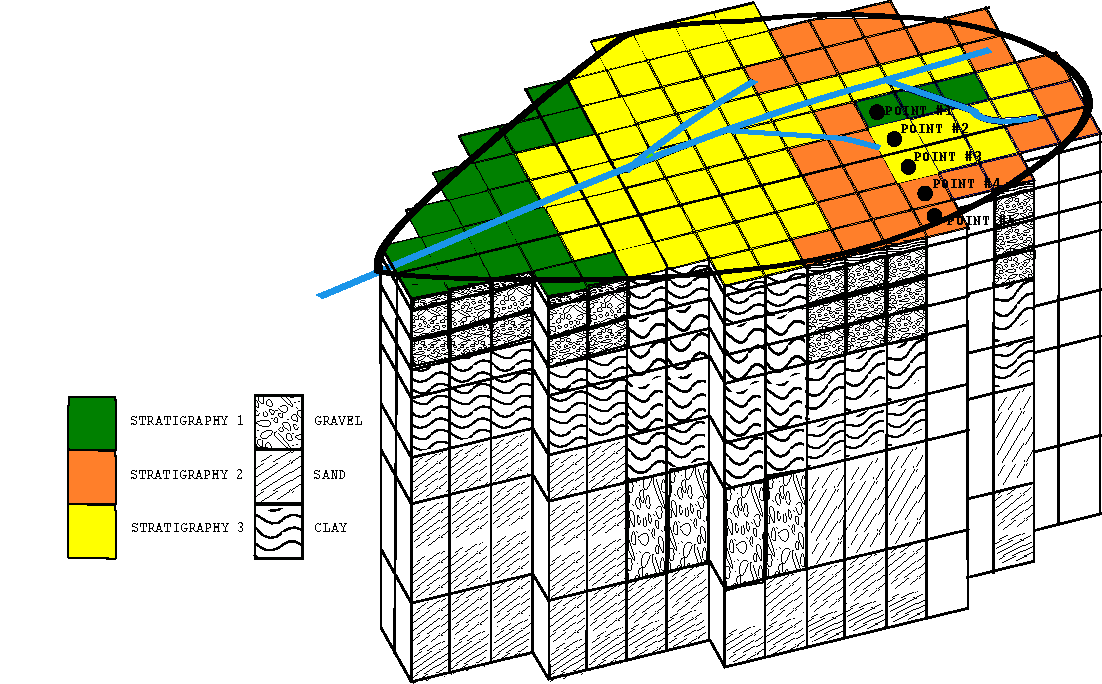
\includegraphics[width=1.8 \textwidth]{./images/pic_domain/soil_type_stratigraphy.pdf}
\end{minipage}
\vspace{10 mm}
\begin{minipage}[c]{0.5 \textheight}
\centering
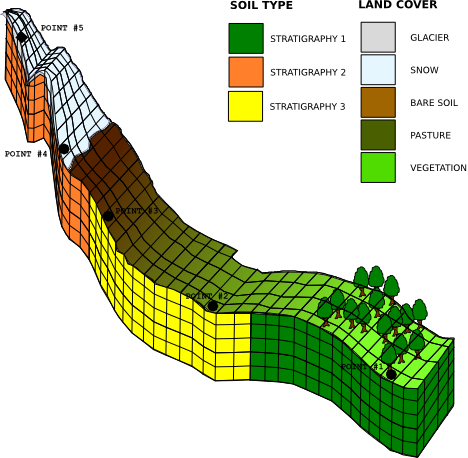
\includegraphics[width=0.9 \textwidth]{./images/pic_domain/grid3Dversante_points}
\end{minipage}
\caption{Domain characterization oriented to define the soil stratigraphy (soil type map).}
\label{grid3Dversante_points}
\end{center}
\end{figure}



%\begin{figure}[!h]
%\begin{center}
%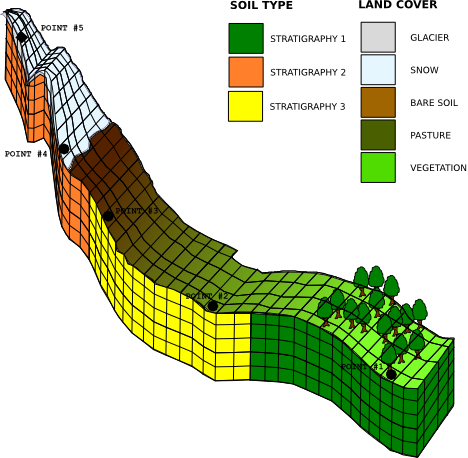
\includegraphics[width=0.8 \textwidth]{./images/pic_domain/grid3Dversante_points}
%\caption{Slope sectio: calculation domain and classification of land surface and soil type. }
%\label{grid3Dversante_points}
%\end{center}
%\end{figure}

\section{The focus on some points}\label{par:focusPoints}

It is possible to select some points in the basin that deserve a special attention, i.e. for the presence of a measurement device or for civil protection reasons. These points may be located wherever in the domain area and may be classified according to topographic characteristics (elevation, slope, aspect), surface type (land cover) and soil stratigraphy (soil type). Table \ref{table_points_charact} summarizes the characteristics of the simulation points reported on Fig. \ref{grid3Dversante_points}. The point 1 is located at low altitude on the bottom valley, in a vegetated area near the channel. The point 2 is located slightly upwards on the pasture, the point 3 is at medium-high altitude, where no vegetation is present (bare soil). The point 4, at 2500 m altitude, is still snow covered and finally the point 5, at 3100 m, is characterized by the presence of a glacier. As far as the soil type is concerned, the slope is characterized by the stratigraphy 1 at low altitude near the channel, where the point 1 is located. Then, at medium-range altitude, it is characterized by the stratigraphy 3 (see points 2 and 3) and finally, at high elevations, by the stratigraphy 2 (points 5 and 6).\\
These points may be highlighted to run multiple 1D simulations (see Par. \ref{par:1D3D}) or to print specific point results.


\begin{center}
\begin{longtable}{|p {1.5 cm}|p {1.5 cm}|p {1.5 cm}|p {1.8 cm}|p {1.8 cm}|p {1.8 cm}|}
\hline
\textbf{Point ID} & \textbf{Elevation (m a.s.l.)} & \textbf{Slope ($^\circ$)} & \textbf{Aspect ($^\circ$ N)} & \textbf{Land cover}& \textbf{Soil type} \\ \hline
\endfirsthead
\hline
\multicolumn{5}{| c |}{continued from previous page} \\
\hline
\textbf{Point ID} & \textbf{Elevation (m a.s.l.)} & \textbf{Slope ($^\circ$)} & \textbf{Aspect ($^\circ$ N)} \textbf{Land cover} & \textbf{Soil type} \\ \hline
\endhead
\hline
\multicolumn{5}{| c |}{{continued on next page}}\\ 
\hline
\endfoot
\endlastfoot
\hline
1 & 1200 & 15 & 30 & vegetation &1  \\ \hline
2 & 1600 & 10 & 30 & pasture &3 \\ \hline
3 & 2200 & 20 & 15 & bare soil  &3\\ \hline
4 & 2500 & 25 & 0 & snow  &2\\ \hline
5 & 3100 & 25 & 0 & glacier &2 \\ \hline
\caption{Topographic, land cover and soil type characteristics of the simulation points}
\label{table_points_charact}
\end{longtable}
\end{center}



\section{Meteorological forcing}

The meteorological data represent the dynamic forcing that constrain the domain to evolve, under the constraints given by topography, the conservation laws and the boundary conditions. GEOtop may receive in input the meteorological data coming from several stations (the number of meteo stations is an input parameter).


\subsection{Meteo station}
In order to describe the characteristics of the meteo stations, it is requested to provide the following information:
\begin{itemize}
\item the number of meteo station;
\item the coordinates (X, Y, Lat, Long) of each meteo station;
\item the elevation;
\item the sky view factor;
\item the standard time difference (of the time records with respect to Greenwich Meridiam Time);
\item the height of the wind speed and air temperature sensors.
\end{itemize}

\noindent Fig. \ref{Fig_meteoST1} shows the planar view of the domain area where three meteo stations (ST) are present: ST1 is located on a high peak, ST2 is on the bottom valley and ST3 is on a medium altitude peak at the lefthand side of the river. The prospect view of the meteo stations is reported in Fig. \ref{Fig_meteoST2}. It is important to note the following: (i) the meteo stations may also be outside of the land cover map, however must be located inside the DEM area; (ii) the sky view factor of the meteo station depends on topography: whereas ST1 has no obstruction because of its high elevation, ST2 is characterized by a big obstruction given by the mountain ranges.
Finally, the zoom in Fig. \ref{Fig_meteoST2} reports a particular of the meteo station: the wind sensor height and the air temperature height must be specified in the model.

\begin{figure}[t,b]
\begin{center}
\begin{minipage}[c]{1.0 \textwidth}
\centering
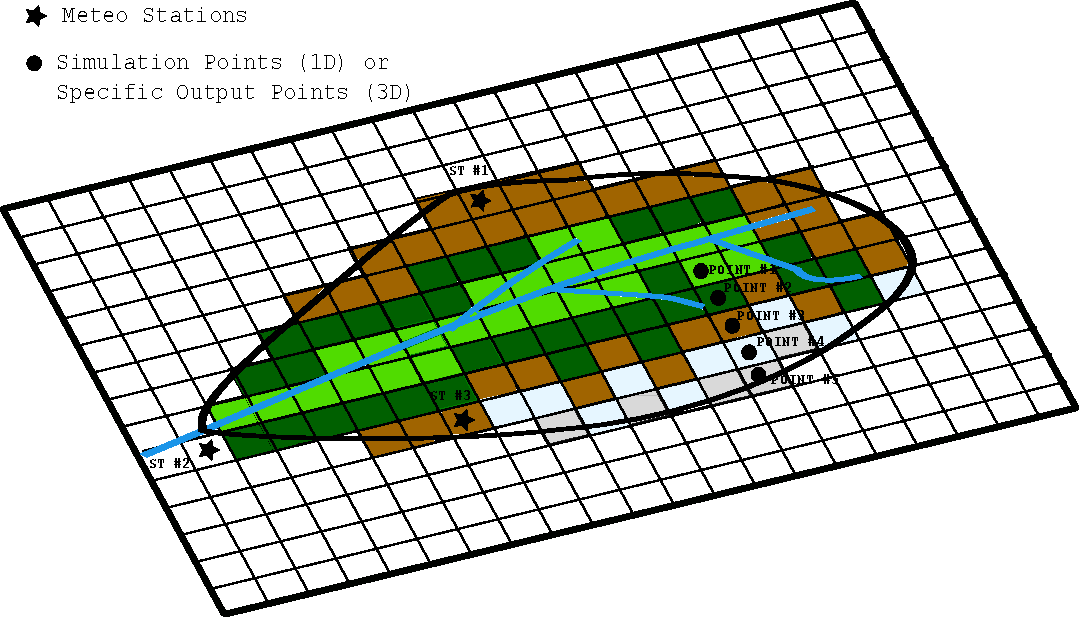
\includegraphics[width =1.0 \textwidth]{./images/pic_domain/foglia_LC_meteo.pdf}
\end{minipage}%
\end{center}
\caption{Planar view of meteo stations (ST) location in the domain area.}
\label{Fig_meteoST1}
\end{figure}


\begin{figure}[t,b]
\centering
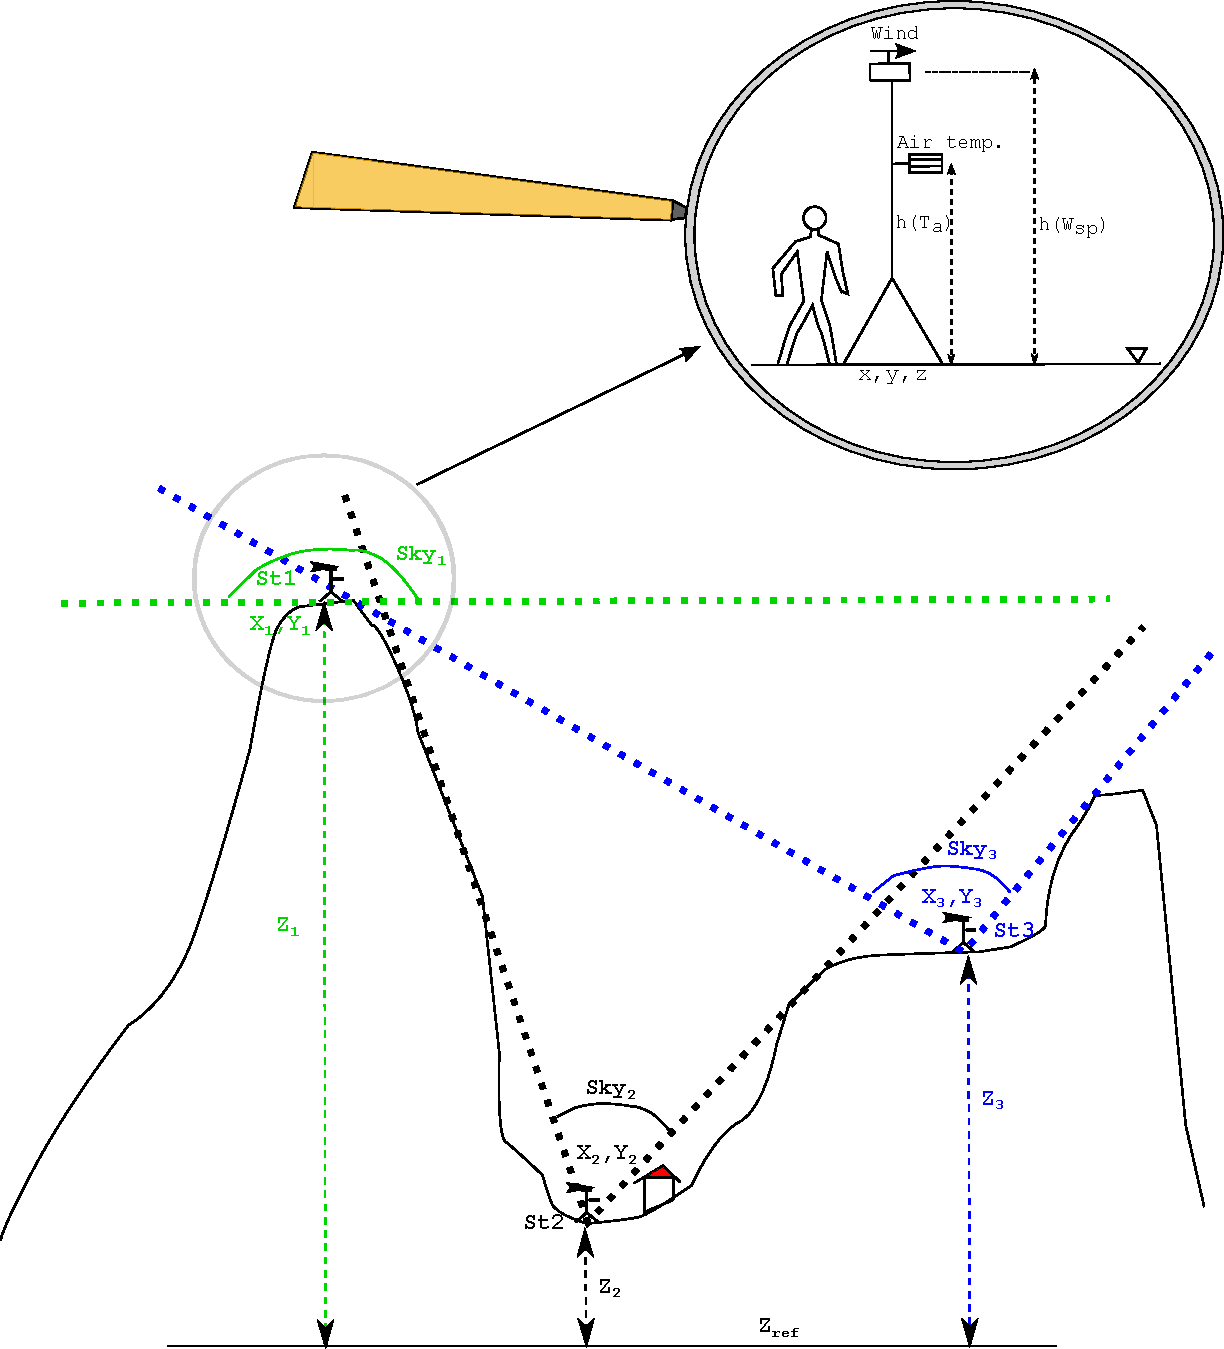
\includegraphics[width =0.85 \textwidth]{./images/pic_domain/MeteoSt.pdf}
\caption{Prospect view of meteo station (ST) location in the domain area. $X, Y, Z$ represent the east coordinate, north coordinate and elevation respectively. In the lence is reported a zoom of one meteo station: $h(T_a)$  and $h(W_{sp})$ represent the height of the air temperature and wind sensor respectively}
\label{Fig_meteoST2}
\end{figure}


\subsection{Meteo data}

Each meteo station, according to the sensor installed, may measure different type of variables. The admitted input variables considered as meteorological forcing are:

\begin{enumerate}
\item precipitation intensity (mm h$^{-1}$)
\item wind velocity (m s$^{-1}$)
\item wind direction ($^\circ$N)
\item windX and windY (m s$^{-1}$) (must belong to the same meteo station) 
\item relative humidity (\%)
\item air temperature ($^\circ$C)
\item dew temperature ($^\circ$C)
\item air pressure (bar)
\item short wave solar global radiation (W m$^{-2}$)
\item short wave solar direct radiation (W m$^{-2}$)
\item short wave solar diffuse radiation (W m$^{-2}$)
\item short wave solar net radiation (W m$^{-2}$)
\item long wave incoming radiation (W m$^{-2}$)
\end{enumerate}

\noindent The meteo variables have to be provided in the Meteo file, specified by the keyword {\it MeteoFile}. 
 It is compulsory to add to the file the column of the date, given by the DD/MM/YYYY hh:mm format or by the Julian day.
 Figg. \ref{meteo_cm1_old}, \ref{meteo_cm2} \ref{meteo_cm3} report an example of the time series that may be given in input.
The {\bf nodata} value is coded through the number {\bf -9999}.

\subsection{Cloudiness}

cloud transmissivity ( - )\\
cloud factor ( - ) 

\subsection{Lapse rates}

The meteorological variables are usually characterized by a gradient on elevation, known as ``lapse rate''. It represents the variation of the variable with elevation. GEOtop admits in input the a dynamic lapse rate that (variable in time) that, according to the elevation of the calculation grid node, modifies the value of the variable. The meteorological variable that admits a lapse rate are:
\begin{itemize}
\item lapse rate for precipitation (mm h$^{-1}$ hm$^{-1}$)\\
\item lapse rate for air temperature ($^\circ$C hm$^{-1}$)\\
\item lapse rate for dew temperature ($^\circ$C hm$^{-1}$)
\end{itemize}


\begin{figure}[t,b]
\centering
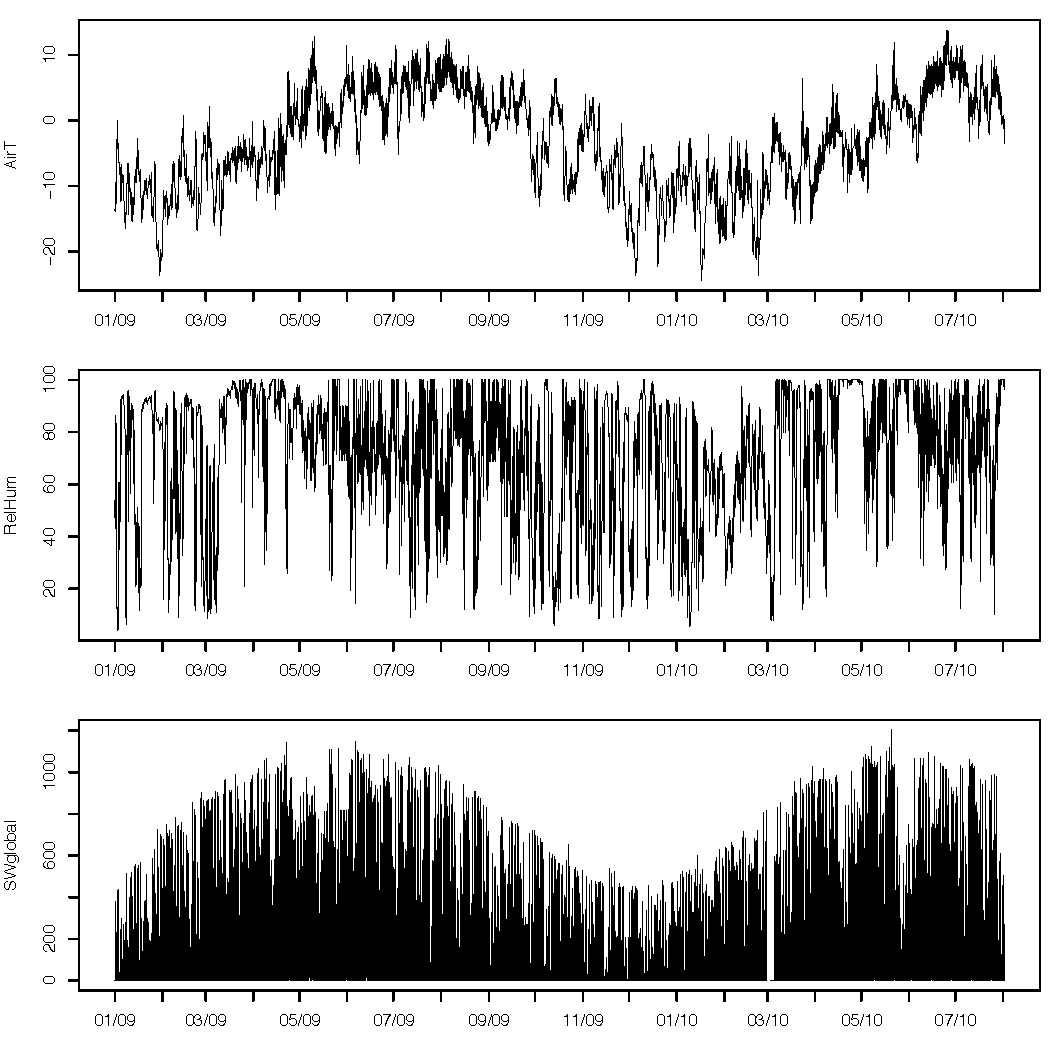
\includegraphics[width =0.9 \textwidth]{./images/pic_domain/meteo_cm1_old.pdf}
\caption{Meteo data measured in a meteo station. Top: air temperature (m s$^{-1}$); middle: relative humidity (\%); bottom: short wave global radiation (W m$^{-2}$)}
\label{meteo_cm1_old}
\end{figure}

\begin{figure}[t,b]
\centering
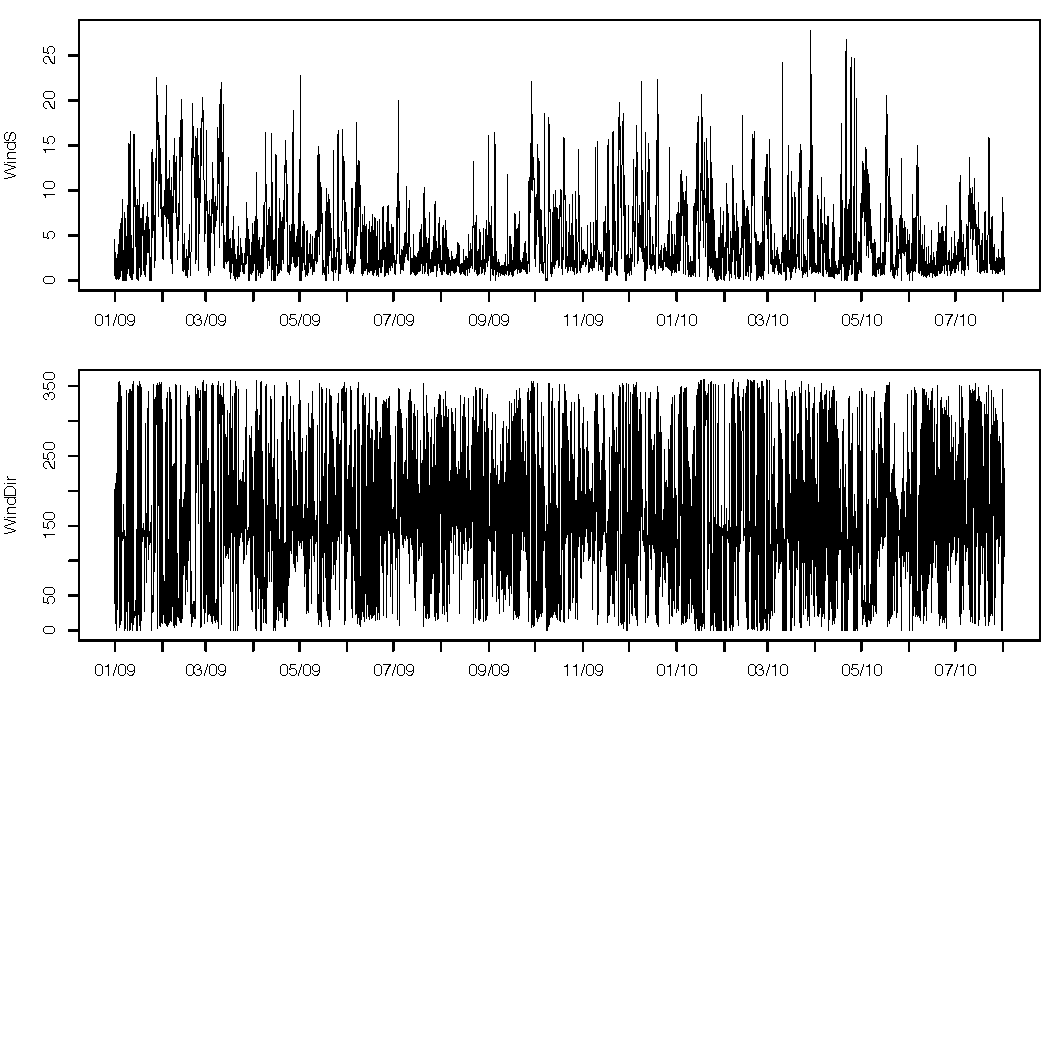
\includegraphics[width =0.9 \textwidth]{./images/pic_domain/meteo_cm2.pdf}
\caption{Meteo data measured in a meteo station. Top: wind speed (m s$^{-1}$); bottom: wind direction ($^\circ$ N)}
\label{meteo_cm2}
\end{figure}

\begin{figure}[t,b]
\centering
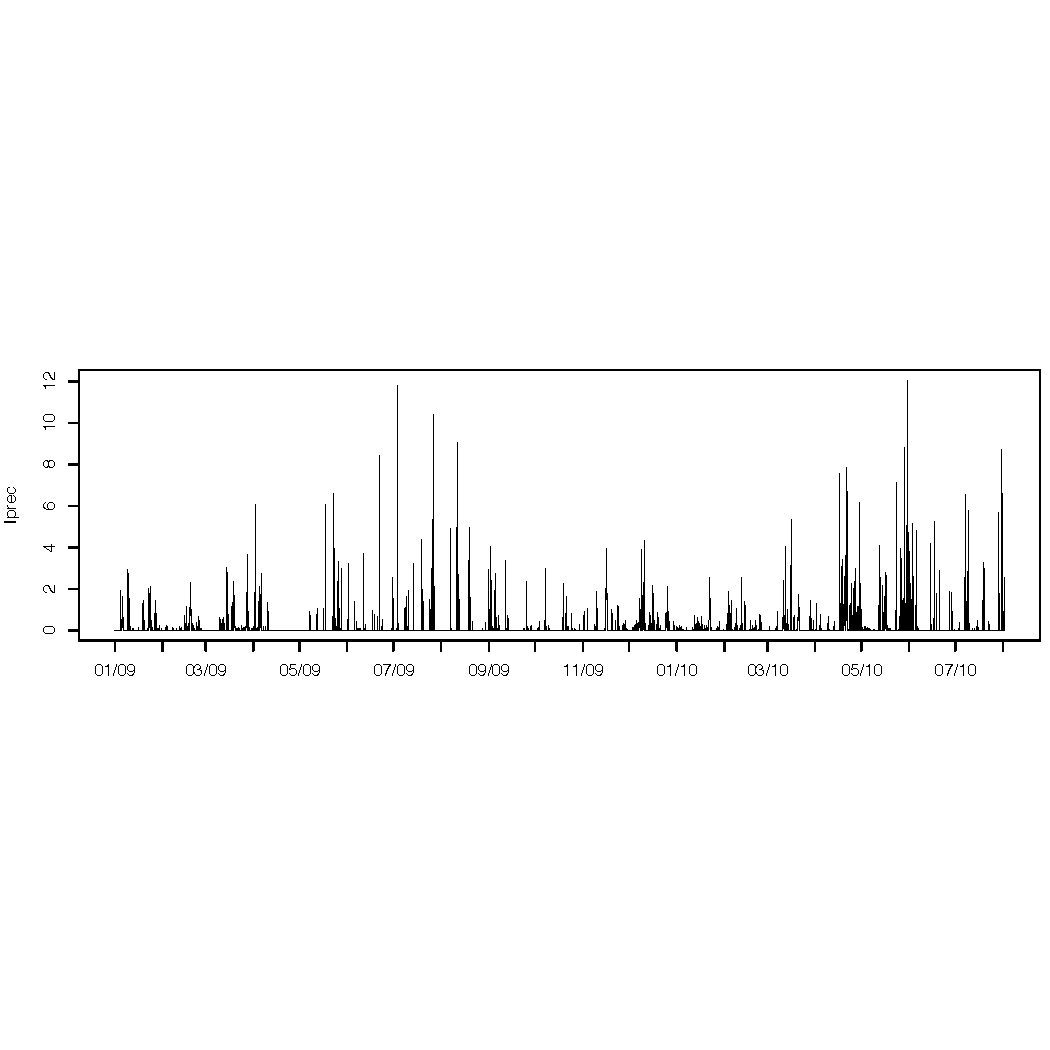
\includegraphics[width =0.9 \textwidth]{./images/pic_domain/meteo_cm3.pdf}
\caption{Meteo data measured in a meteo station: precipitation intensity (mm h$^{-1}$)}
\label{meteo_cm3}
\end{figure}
